\vspace*{20\baselineskip}
\section{Faltungscodes}
\begin{center}
    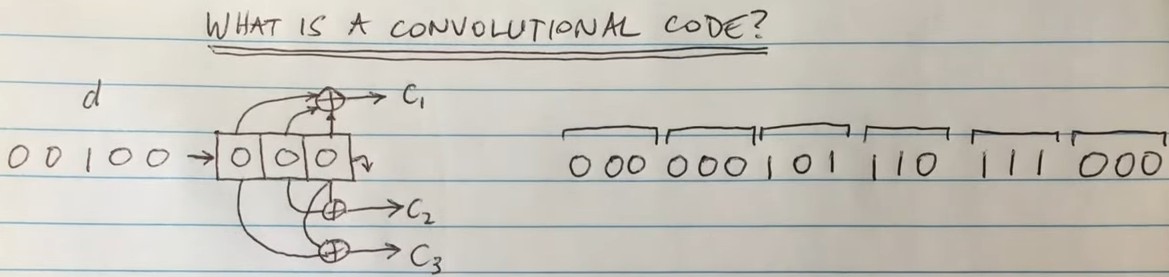
\includegraphics[scale=0.31]{faltungscode}
\end{center}
\subsection{Trellis Diagramm}
Ein Trellis Diagramm ist eine graphische Darstellung eines Faltungscodes. 
Jeder Knoten repräsentiert einen Zustand und jede Kante eine mögliche Transition.
Ein Codewort muss man Rückwärts durch den Baum laufen lassen, um den ursprünglichen Zustand zu finden.

\begin{center}
    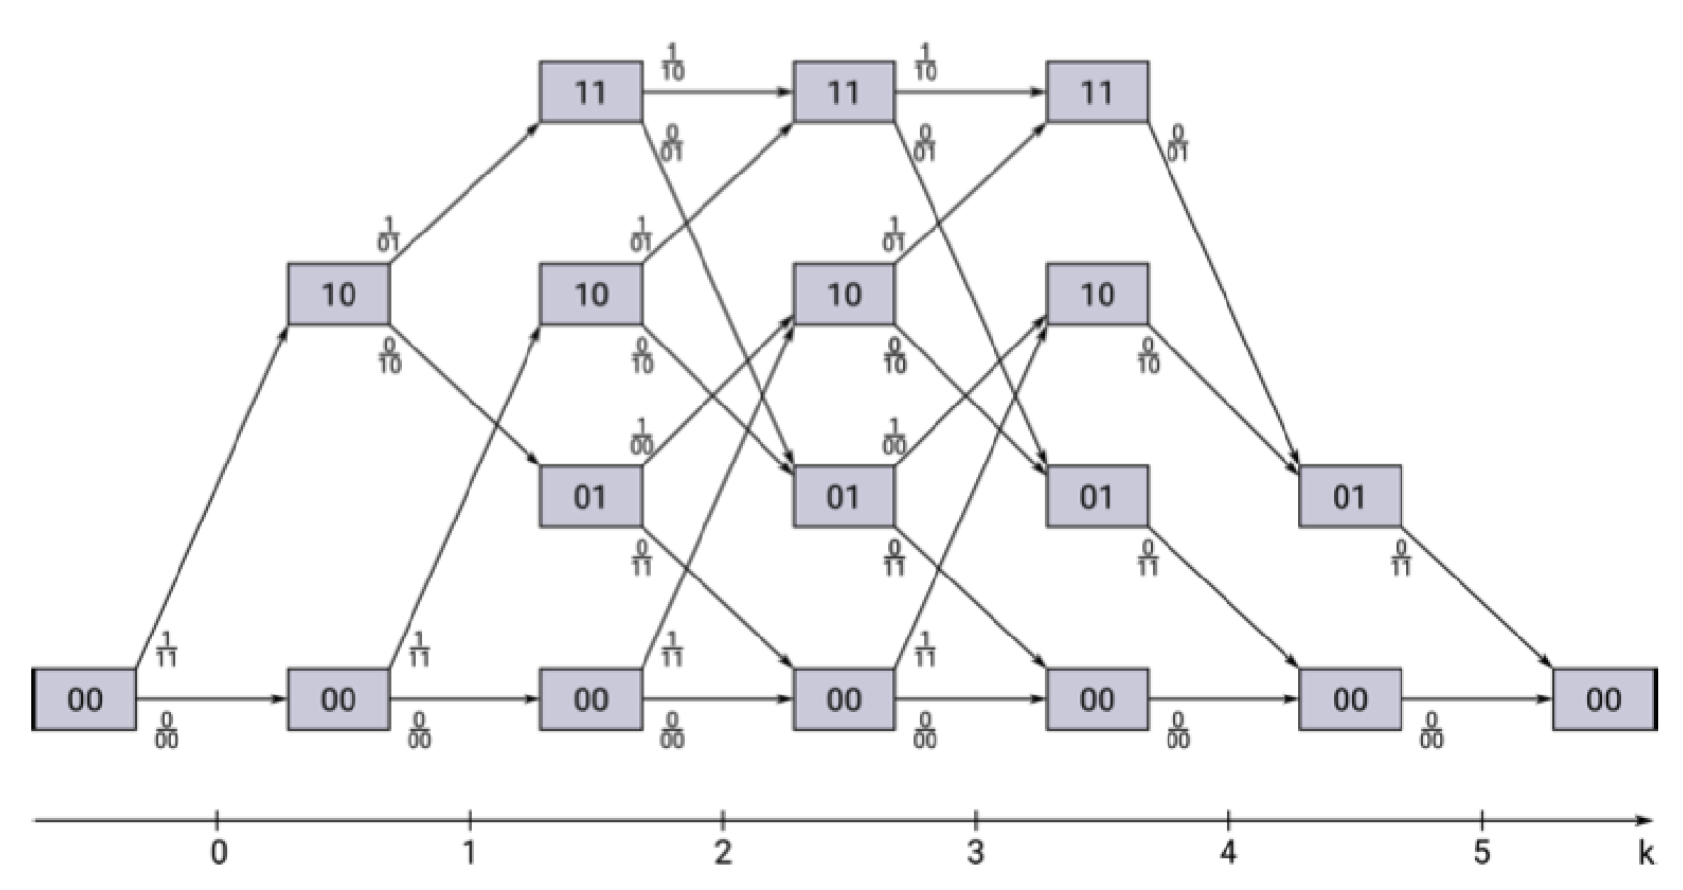
\includegraphics[scale=0.2]{trellis}
\end{center}
\subsection{Optimum Free Distance}
\begin{align*}
    d_{free} = W_{min}
\end{align*}
\\
$W_{min}$ ist das minimale Hamming Gewicht. Berechnung, in dem von
Zustand $[000]$ gestartet wird und der kürzeste Weg zurückgenommen wird.
\begin{center}
    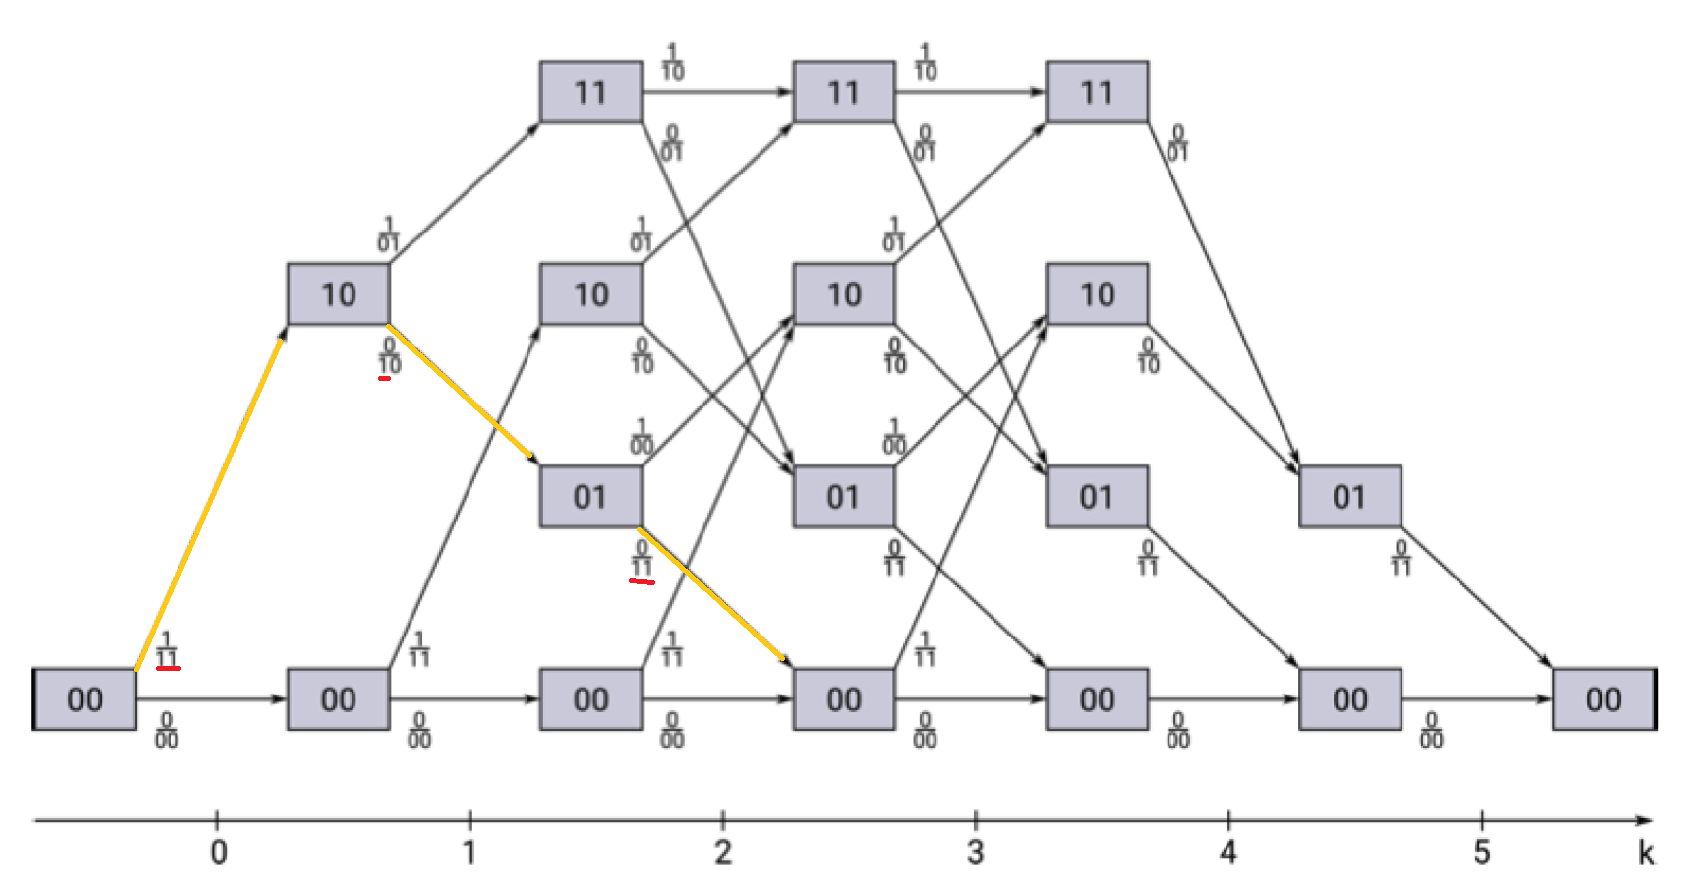
\includegraphics[scale=0.2]{trellis1}
\end{center}
Die Anzahl der Einsen auf dem kürzesten Weg ist $W_{min} = 5$.

\subsection{Coderate $R$}
\begin{align*}
    R = \frac{K}{N} = \frac{K}{2 \cdot (K + m)}
\end{align*}
\subsubsection{Tailbits $m$}
Tailbits sind die $m$ Bits am Ende der Nutzdatenvektoren. Sie sind notwendig, um den Codierer in den 
Anfangszustand zurückzuführen.
\begin{center}
    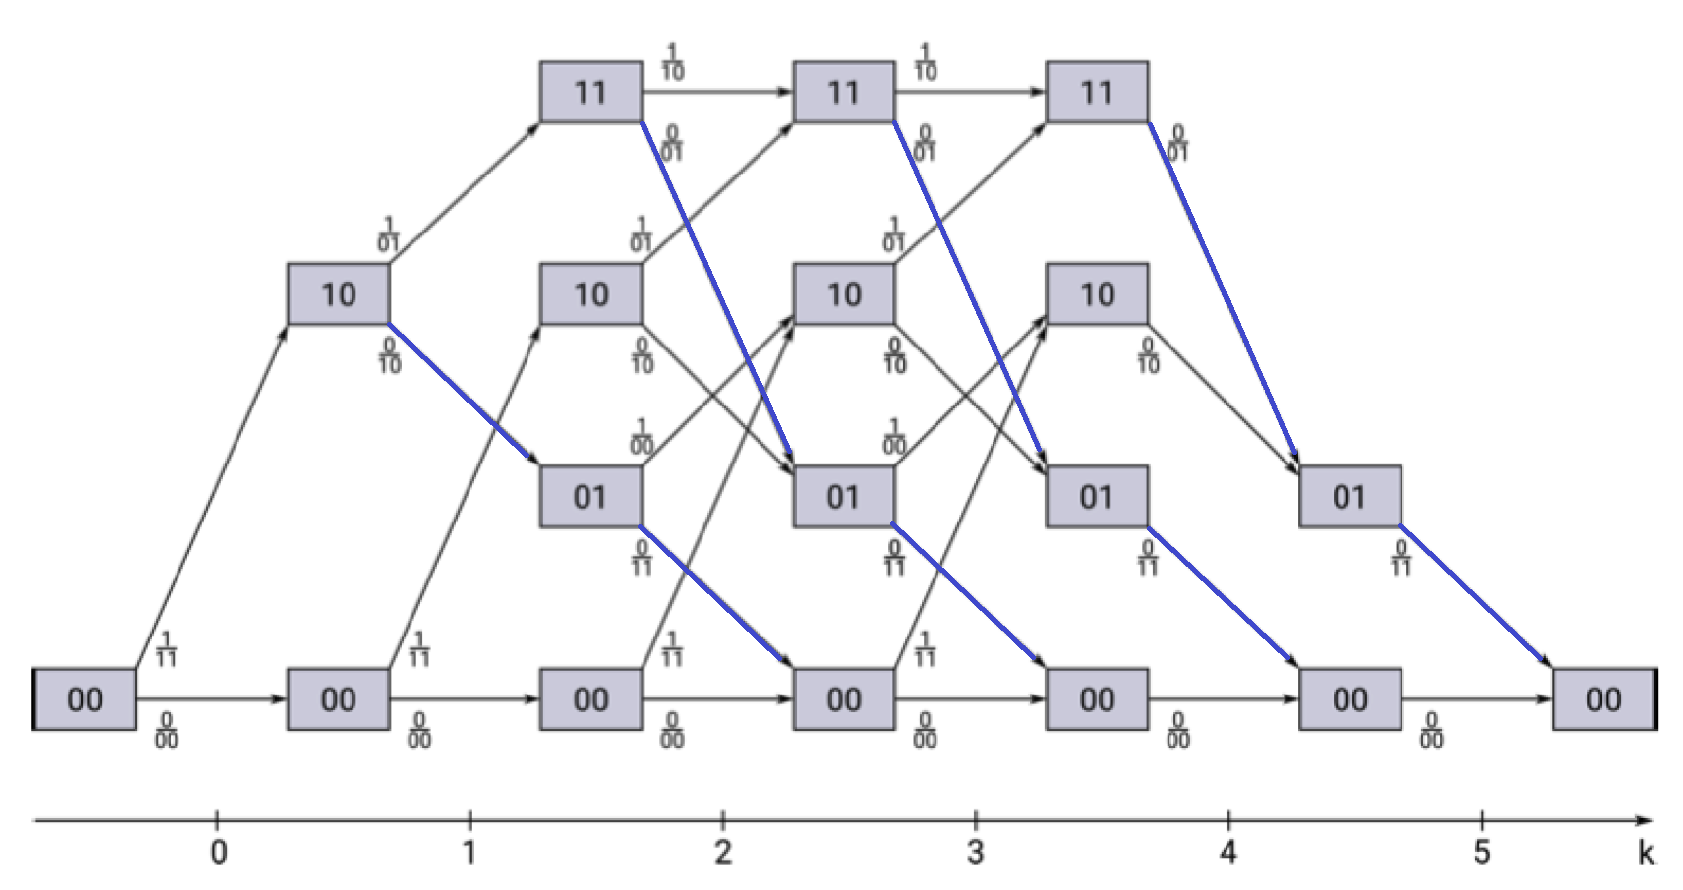
\includegraphics[scale=0.2]{trellis2}
\end{center}
Die Anzahl Tailbits $m$ ist Wie viele Schritte benötigt werden, um von einem 
Zustand in den Anfangszustand zurückzukehren. In diesem Fall sind es $2$ Schritte.